\documentclass[]{achemso}

\usepackage{amsmath}        % Equation editing using flags of \begin{align} and \end{align}
\usepackage{commath}        % We have this here to use the \abs{} equation function
\usepackage{graphicx}       % Display figures using \includegraphics
\graphicspath{{figures/}}   % Location for figures relative to .tex file path
\usepackage{booktabs}       % Use table things like \toprule or \bottomrule
\usepackage[table]{xcolor}  % Lets us use \rowcolors to make alternate table shading
\usepackage{makecell}       % Allow the use of the \makecell command that lets linebreaks in table cells
\usepackage{etoolbox}       % Make the bibliograph unjustified (to work around hbox errors)
\apptocmd{\thebibliography}{\raggedright}{}{}
\usepackage{glossaries}     % Enable the \newacronym and \gls commands to reference terms

\newacronym{DFT}{DFT}{Density Functional Theory}
\newacronym{VASP}{VASP}{the Vienna Ab-initio Simulation Package}
\newacronym{GASpy}{GASpy}{the Generalized Adsorption Simulator for Python}
\newacronym{rPBE}{rPBE}{revised Perdew-Burke-Ernzerhof}
\newacronym{ASE}{ASE}{the Atomic Simulation Environment}
\newacronym{NEB}{NEB}{nudged elastic band}
\newacronym{GP}{GP}{Gaussian Process}
\newacronym{UQ}{UQ}{uncertainty quantification}
\newacronym{MAE}{MAE}{Mean Absolute Error}
\newacronym{RMSE}{RMSE}{Root Mean Squared Error}
\newacronym{MDAE}{MDAE}{Median Absolute Error}
\newacronym{MARPD}{MARPD}{Mean Absolute Relative Percent Difference}
\newacronym{R2}{R\textsuperscript{2}}{R\textsuperscript{2} correlation coefficient}
\newacronym{Pearson}{Pearson's}{Pearson product-moment correlation coefficent}
\newacronym{CGCNN}{CGCNN}{Crystal Graph Convolutional Neural Network}
\newacronym{BNN}{BNN}{Bayesian Neural Network}
\newacronym{MLE}{MLE}{Maximum Likelihood Estimation}
\newacronym{PFGP}{PFGP}{Penultimate-Fed Gaussian Process}
\newacronym{ML}{ML}{Machine Learning}


%%%%%%%%%%%%%%%%%%%% Title/Abstract %%%%%%%%%%%%%%%%%%%%
\title{Uncertainty quantification in deep networks for material property predictions}
\author{Kevin Tran}
\affiliation{Chemical Engineering Department, Carnegie Mellon University, Pittsburgh, PA 15217}
\altaffiliation{These authors contributed equally to this work}
\author{Willie Neiswanger}
\affiliation{Machine Learning Department, Carnegie Mellon University, Pittsburgh, PA 15217}
\altaffiliation{These authors contributed equally to this work}
\author{Junwoong Yoon}
\affiliation{Chemical Engineering Department, Carnegie Mellon University, Pittsburgh, PA 15217}
\author{Eric Xing}
\affiliation{Machine Learning Department, Carnegie Mellon University, Pittsburgh, PA 15217}
\author{Zachary W. Ulissi}
\affiliation{Chemical Engineering Department, Carnegie Mellon University, Pittsburgh, PA 15217}
\email{zulissi@andrew.cmu.edu}

\begin{document}

%\setlength{\fboxrule}{0 pt}
%\begin{tocentry}
%    \includegraphics[width=\textwidth]{TOC/TOC.pdf}
%    TOC caption here.
%\end{tocentry}

\begin{abstract}
    Abstract here.
\end{abstract}


%%%%%%%%%%%%%%%%%%%% Introduction %%%%%%%%%%%%%%%%%%%%

\section{Introduction}

The fields of catalysis and materials science are burgeoning with methods to screen, design, and understand materials.\cite{Medford2018, Gu2019, Schleder2019, Alberi2019}
This research has spurned the creation of \gls{ML} models to predict various material properties.
Unfortunately, the design spaces for these models are sometimes too large and intractable to sample completely.
These undersampling issues can limit the training data and therefore the predictive power of the models.
It would be helpful to have an \gls{UQ} for a model so that we know when to trust the predictions and when not to.
More specifically:  \gls{UQ} would enable various online, active frameworks for materials discovery and design (e.g., active learning,\cite{Settles2012} online active learning,\cite{Chu2011} Bayesian optimization,\cite{Frazier2018} active search,\cite{Garnett2012} or goal oriented design of experiments\cite{Kandasamy}).

Such active frameworks have already been used successfully in the field of catalysis and materials informatics.
For example:  \citet{Peterson2016} has used a neural network to perform online active learning of \gls{NEB} calculations, reducing the number of force calls by an order of magnitude.
\citet{Torres2018} have used also used online active learning to accelerate \gls{NEB} calculations, but they used a \gls{GP} model instead of a neural network.
\citet{Jinnouchi2019} have used online active learning to accelerate molecular dynamics simulations.
Each of these active methods are underpinned by models with \gls{UQ}, which has garnered increasing attention itself.\cite{Peterson2017, Musil2019}

% TODO: Willie to make overview of predictive uncertainty

To our knowledge though, we have not seen many comparisons of different methods for \gls{UQ} within the field of catalysis and materials informatics.
Here we attempt to resolve this issue by benchmarking six different methods for \gls{UQ} (Figure~\ref{fig:overview}).
We acknowledge that there will not be one optimal method across all use cases, but we still find value in sharing these results so that others can build intuition from our results.
Perhaps more importantly, we have also established a protocol for comparing the performance of different modeling and \gls{UQ} methods.

% TODO:  Kevin to make this figure
\begin{figure}
    \centering
    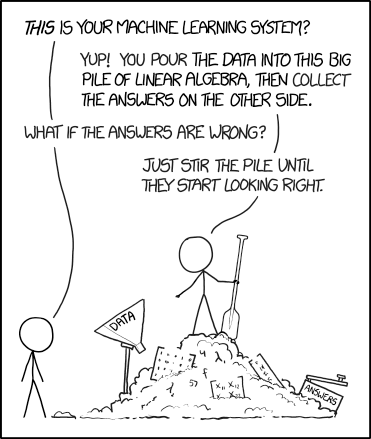
\includegraphics[width=0.5\textwidth]{placeholder.png}
    \caption{Placeholder for overview of the paper}\label{fig:overview}
\end{figure}


%%%%%%%%%%%%%%%%%%%% Methods %%%%%%%%%%%%%%%%%%%%

\section{Methods}

\subsection{Data handling}

All regressions in this paper were performed on a dataset of \gls{DFT} calculated adsorption energies created with \gls{GASpy}\cite{Tran2018, Tran2018a}.
These data included energies from 21,269 different H adsorption sites; 1,594 N sites; 18,437 CO sites; 2,515 O sites; and 3,464 OH sites; totaling in 47,279 data points.
\gls{GASpy} performed all \gls{DFT} calculations using \gls{VASP}\cite{Kresse1993, Kresse1994, Kresse1996, Kresse1996a} version 5.4 implemented in \gls{ASE}\cite{HjorthLarsen2017}.
The \gls{rPBE} functionals\cite{Hammer1999} were used along with \gls{VASP}'s pseudopotentials, and no spin magnetism or dispersion corrections were used.
Bulk relaxations were performed with a $10\times10\times10$ k-point grid and a 500 eV cutoff, and only isotropic relaxation were allowed during this bulk relaxation.
Slab relaxations were performed with k-point grids of $4\times4\times1$ and a 350 eV cutoff.
Slabs were replicated in the X/Y directions so that each cell was at least 4.5 \AA{} wide, which reduces adsorbate self-interaction.
Slabs were also replicated in the Z direction until they were at least 7 \AA{} thick, and at least 20 \AA{} of vacuum was included in between slabs.
The bottom layers of each slab were fixed and defined as those atoms more than 3 \AA{} from the top of the surface in the scaled Z direction.

To split the data into train/validate/test sets, we enumerated all adsorption energies on monometallic slabs and added them to the training set manually. 
We did this because some of the regression methods in this paper use a featurization that contains our monometallic adsorption energy data\cite{Tran2018}, and so having the monometallic adsorption energies pre-allocated in the training set prevented any information leakage between the training set and validation/test sets.
After this allocation, we performed a 64/14/20 train/validate/test split that was stratified\cite{Thompson2012} by adsorbate.
We then used the validation set's results to tune various hyperparameters manually.
After tuning, we calculated the training set results and present them in this paper exclusively.

\subsection{Regression methods}

% TODO:  Willie to make intro to predictive uncertainty methods.
Figure~\ref{fig:methods} illustrates all the methods we investigated in this study.

\begin{figure}
    \centering
    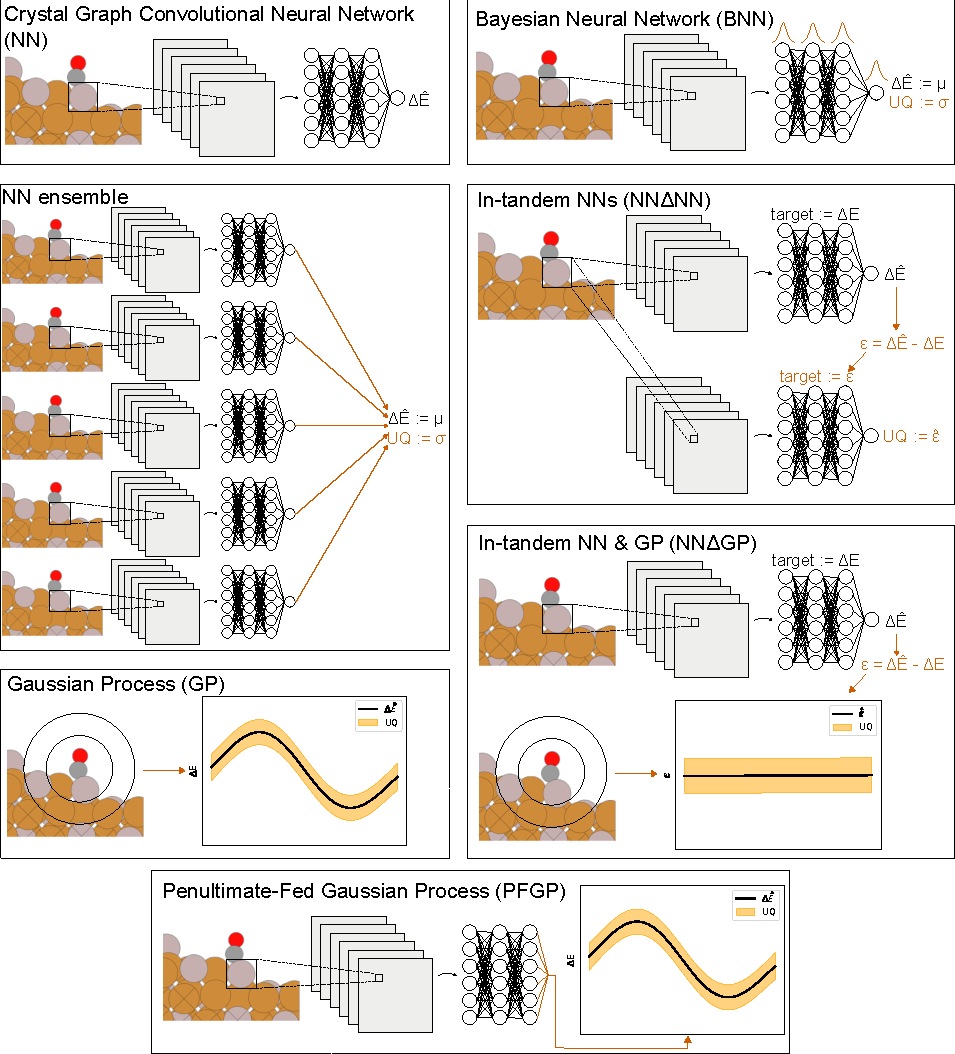
\includegraphics[width=0.8\textwidth]{methods.pdf}
    \caption{Overview of the various \gls{UQ} methods we investigated in this study.
        $\Delta E$ represents \gls{DFT}-calculated adsorption energies;
        $\Delta \hat{E}$ represents \gls{ML}-predicted adsorption energies;
        $UQ$ represents \gls{ML}-predicted uncertainty quantifications;
        $\mu$ represents the mean of a sample of points;
        $\sigma$ represents the standard deviation of a sample of points;
        $\epsilon$ represents the residuals between \gls{DFT} and \gls{ML};
        and $\hat{\epsilon}$ represents the residuals between \gls{ML}-predicted $\epsilon$ and the actual $\epsilon$.
    }\label{fig:methods}
\end{figure}

\textbf{\gls{CGCNN}:}
To establish a baseline for predictive accuracy, we re-trained a previously reported \gls{CGCNN}\cite{Xie2018, Back2019} on this study's training set.
This \gls{CGCNN} model projects a three-dimensional atomic structure into a graph, which is then fed into a convolutional neural network to predict various properties.
In this case, we predict \gls{DFT}-calculated adsorption energies, $\Delta$E.
Reference \citet{Back2019} for additional details.

\textbf{\gls{CGCNN} Ensemble:}
We created an ensemble of \gls{CGCNN}s by K-fold subsampling the training data into five different folds and then training individual \gls{CGCNN} models on each of these folds.
Thus the mean of each of these models' predictions is the final prediction of the ensemble, and the standard deviation of the individual predictions is the ensemble's estimate of uncertainty.
% TODO:  Willie to provide justification for subsampling method. And maybe a reference for K-folding?

\textbf{\gls{BNN}:}
% TODO:  Jun

\textbf{Supervised error prediction (delta CGCNN):}
% TODO:  Willie

\textbf{\gls{GP}:}
\gls{GP}s are one of the most common regression methods for producing \gls{UQ}s, and so we use them here as a baseline.
We fit a standard \gls{GP} using the same exact features that we used in previous work.\cite{Tran2018}
These features are defined by the elements coordinated with the adsorbate and by the elements of its next-nearest neighbors.
Specifically:  We use the atomic numbers of these elements, their Pauling electronegativity, a count of the number of atoms of each element near the adsorbate, and the median adsorption energy between the adsorbate and the elements.
To ensure that these features interacted well with the \gls{GP}'s kernel, we normalized each of the features to have a mean of zero and standard deviation of one.
Reference \citet{Tran2018} for additional details.
To define the GP, we assumed a constant mean and used a Matern covariance kernel.
We trained the length scale of the Matern kernel using the \gls{MLE} method with a Gaussian likelihood.
All GP training and predictions were done with GPU acceleration as implemented in GPyTorch.\cite{Gardner2018}.
% TODO:  Willie double-check the wording here. I think we use a Gaussian likelihood, but does make it no longer MLE? You know best.

\textbf{\gls{GP} with \gls{CGCNN}-predicted mean:}
% TODO:  Willie

\textbf{\gls{PFGP}:}
A limitation of using this formulation of a \gls{GP} with \gls{CGCNN}-predicted mean is that it requires the use of hand-crafted features for the \gls{GP}.
This requirement reduces the transferability of the method to other applications where such features may not be readily available.
To address this, we formulated a different method whereby we first train a neural network on the learning task (i.e., predict adsorption energies), and then we use the outputs of the penultimate layer of the network as features in a new \gls{GP}.
The \gls{GP} would then be trained to use these features to produce both mean and uncertainty predictions on the adsorption energies.
We call this a \gls{PFGP}.
In this case, we used the baseline \gls{CGCNN} as the network from which we obtained the penultimate outputs.
We also normalized the penultimate outputs of the \gls{CGCNN} so that each output would have a mean of zero and a standard deviation of one.
To define the \gls{GP}, we assumed a constant mean and used a Matern covariance kernel.
We trained the length scale of the Matern kernel using the \gls{MLE} method with a Gaussian likelihood.
All GP training and predictions were done with GPU acceleration as implemented in GPyTorch.\cite{Gardner2018}.
% TODO:  Willie double-check the wording here. I think we use a Gaussian likelihood, but does make it no longer MLE? You know best.


\subsection{Performance metrics}

We used six different metrics to quantify the accuracy of the various models:  \gls{MAE}, \gls{RMSE}, \gls{MDAE}, \gls{MARPD}, \gls{R2}, and \gls{Pearson}.
\gls{MARPD} values were calculated with Equation~\ref{eq:marpd}

\begin{equation}\label{eq:marpd}
    MARPD = \frac{1}{N} \sum_{i=1}^{N} \abs{100 \cdot \frac{\hat{x}_n - x_n}{\abs{\hat{x}_n} + \abs{x_n}}}
\end{equation}

\noindent where $n$ is the index of a data point, $N$ is the total number of data points, $x_n$ is the true value of the data point, and $\hat{x}_n$ is the model's estimate of $x_n$.
In this case, $x_n$ is a DFT-calculated adsorption energy and $\hat{x}_n$ is the surrogate-model-calculated adsorption energy.
We used \gls{MDAE} because is insensitive to outliers and is therefore a good measure of accuracy for the majority of the data.
We used \gls{RMSE} because it is sensitive to outliers and is therefore a good measure of worst-case accuracy.
We used \gls{MAE} because it lies between \gls{MDAE} and \gls{RMSE} in terms of sensitivity to outliers.
We used \gls{MARPD}, \gls{R2}, and \gls{Pearson} because they provide normalized measures of accuracy that may be more interpretable for those unfamiliar with adsorption energy measurements in eV.
The ensemble of these metrics provide a more robust view of accuracy than any one metric can provide alone.

To assess the calibration (or ``honesty'') of these models' UQs, we created calibration curves. A calibration curve ``displays the true frequency of points in each [prediction] interval relative to the predicted fraction of points in that interval'', as outlined by \citet{Kuleshov2018}.
In other words:  We used the standard deviation predictions to create Gaussian-shaped prediction intervals around each test point, and then we compared these intervals to the models' residuals at these points.
If the residuals tended to fall outside the prediction intervals too often, then the UQs were considered overconfident.
If the residuals tended to fall inside the prediction intervals too often, then the UQs were considered underconfident.
Thus ``well-calibrated'' models had residuals that created a Gaussian distribution whose standard deviation was close to the model's predicted standard deviations.
We discuss calibration curves in more detail in the Results section alongside specific examples.

As \citet{Kuleshov2018} also pointed out, well-calibrated models are necessary but not sufficient for useful UQs.
For example:  A well-calibrated model could still have large uncertainty estimates, which are inherently less useful than well-calibrated and small uncertainty estimates.
This idea of having small uncertainty estimates is called ``sharpness'', and \citet{Kuleshov2018} define it with Equation~\ref{eq:og_sharpness}

\begin{equation}\label{eq:og_sharpness}
    sha = \frac{1}{N} \sum_{n=1}^{N} var(F_n)
\end{equation}

\noindent where $var(F_n)$ is the variance of the cumulative distribution function $F$ at point $n$.
This is akin to the average variance of the uncertainty estimates on the test set.
Here we propose and use a new formulation (Equation~\ref{eq:sharpness}) where we add a square root operation.
This operation gives the sharpness the same units as the predictions, which provides us with a more intuitive reference in the magnitude of the sharpness values.

\begin{equation}\label{eq:sharpness}
    sha = \sqrt{\frac{1}{N} \sum_{n=1}^{N} var(F_n)}
\end{equation}


%%%%%%%%%%%%%%%%%%%% Results %%%%%%%%%%%%%%%%%%%%

\section{Results}

\begin{enumerate}
    \item{Table/figure of metrics}
    \item{Plots:}
        \begin{enumerate}
            \item{parity}
            \item{calibration}
            \item{sharpness}
        \end{enumerate}
    \item{Blocking results on best candidates (maybe put in SI)}
    \item{Cost of computing each method (if it’s there)}
    \item{Human overhead and difficulty}
\end{enumerate}


%%%%%%%%%%%%%%%%%%%% Conclusions %%%%%%%%%%%%%%%%%%%%

\section{Conclusions}

% TODO:  Kevin Observations about relative accuracies, calibrations, sharpnesses, overhead. Note that we did not do any calibration, and possibly provide references on how to do that if you wanted to.


%%%%%%%%%%%%%%%%%%%% Misc %%%%%%%%%%%%%%%%%%%%

\section*{Code availability} Visit \texttt{https://github.com/ulissigroup/uncertainty\_benchmarking} for the code used to create the results discussed in this paper.
The code dependencies are listed inside the repository.

\section*{Author information} Corresponding author email:  zulissi@andrew.cmu.edu.
The authors declare no competing financial interest.

\section*{Acknowledgements} This research used resources of the National Energy Research Scientific Computing Center, a DOE Office of Science User Facility supported by the Office of Science of the U.S. Department of Energy under Contract No. DE-AC02-05CH11231. % chktex 8
We also acknowledge the exceptional documentation and clear examples in the GPyTorch\cite{Gardner2018} repository, which formed the basis on much of the \gls{GP} code used for this work.


%%%%%%%%%%%%%%%%%%%% Bibliography %%%%%%%%%%%%%%%%%%%%

\clearpage
\bibliography{uncertainty_benchmarking}

\end{document}
